\section{Cloud computing}
La computación en la nube es una metáfora para abastecimiento y consumición de recursos de infraestructura. El nivel de abstracción ofrecida por la nube puede variar de hardware virtual a complejos sistemas distribuidos, debido a que los recursos están disponibles a demanda en enormes cantidades y pagados por uso \citep{wittig_amazon_2016}. Casi toda solución de infraestructura remota es basada hoy día con esta tecnología.

La infraestructura remota o nube puede ser manejada por una organización abierta para uso público, o puede ser privada, donde una nube que virtualiza y comparte la infraestructura con una sola organización o híbrida como son mostrados en la figura \ref{cloud_types}.

\begin{figure}[H]
\centering
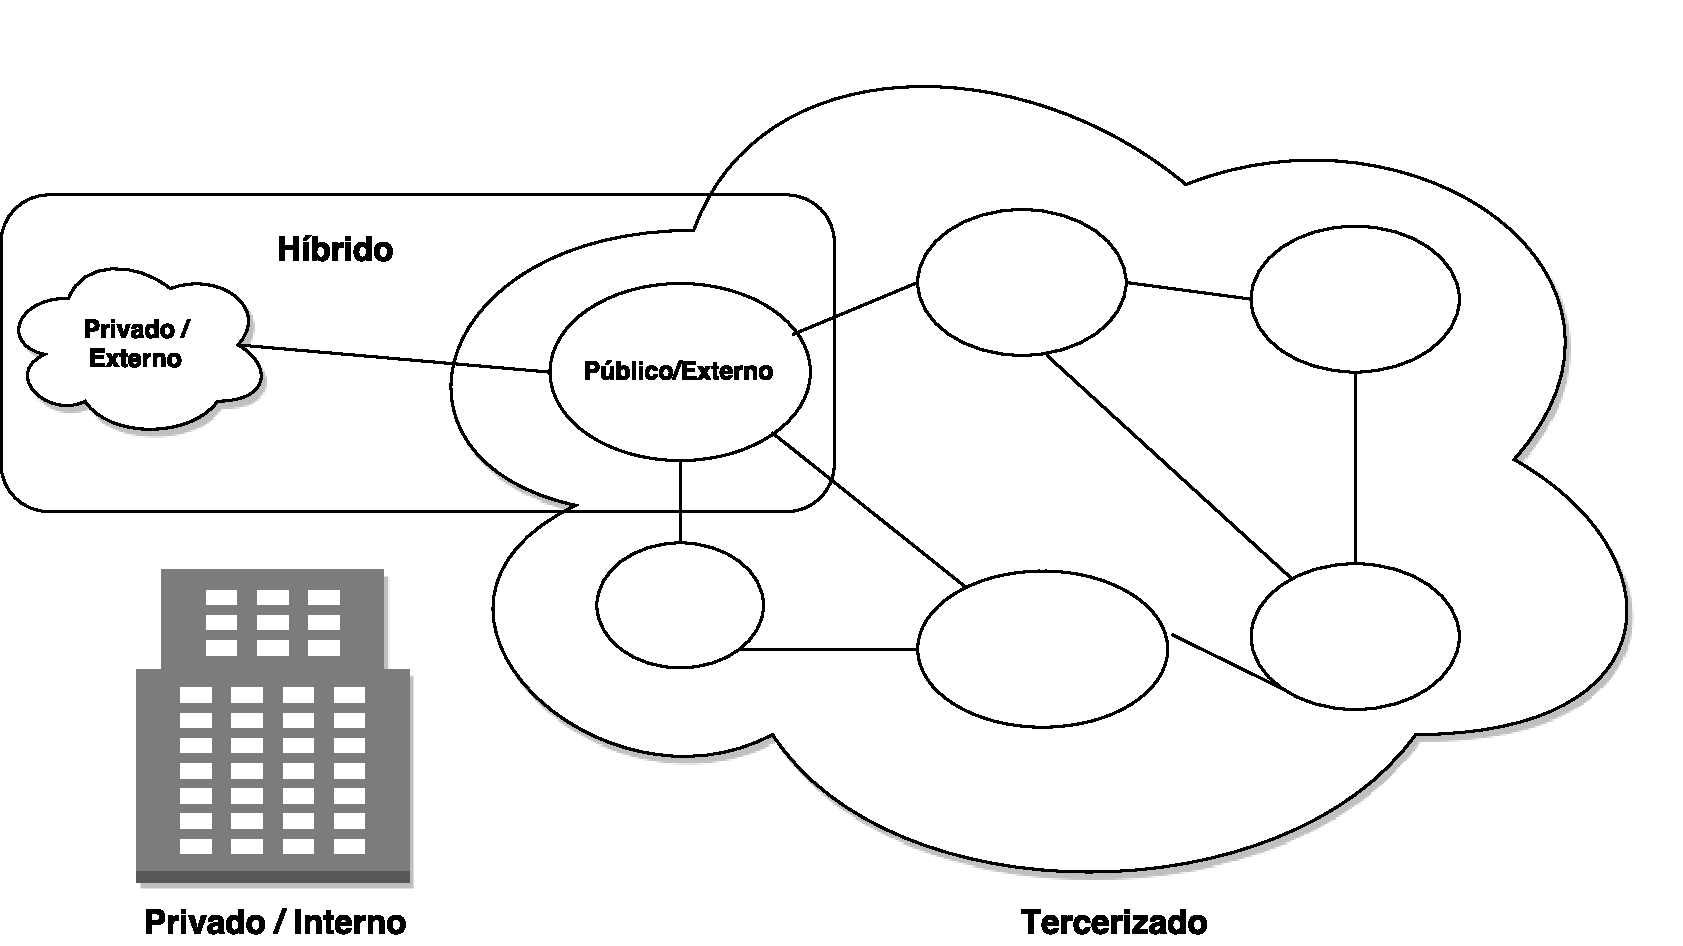
\includegraphics[width=125mm,scale=1]{Figuras/cloud_computing_types}
\caption{Esquema de tipos de computación en la nube.}
  \label{cloud_types}
\end{figure}